\section{Feedback for tracking methods} \label{sec:feedback}

As previously shown in the Fig. \ref{figurelabel_sys} the acquired knowledge by the segmentation mask, and flow estimation can be used to 
feedback the tracker method, and generate a more precise position of the object in the next frame. There are several ways to perform this feedback 
depending on the specific tracking method used. However, to mantain certain generality in the pipeline of the object flow, the used cues are the ones 
given by the segmentation mask and the tracked background regions that could behave as occlusions. 
In the most of the tracking by detection methods, a sampling step (which can be explicit like in the {\it MIL} tracker, or implicit, 
like in the {\it Struck} tracker) is performed to extract features that are valid as possible to represent the target object. 
   
When occlusions happen, the most of the methods have a hard time to select a correct bag of features to represent the said object, as it gets difficult 
for the learning method to explain the object after and before occlusions with a given set of features. The Fig. \ref{tr_mil} shows how Online Adaboost 
and Online Multiple Instance Learning try to deal with this problem when a small occlusion happens. 

   \begin{figure}[thpb]
      \centering
      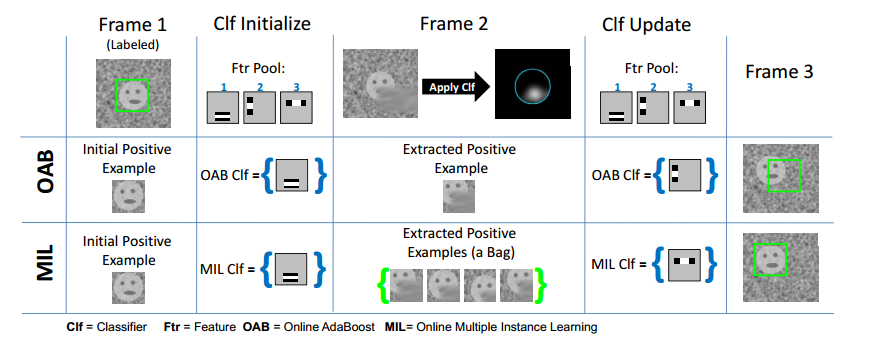
\includegraphics[width=0.85\textwidth]{../images/mil.png}
      \caption{An overview on how tracking-by-detection methods try to deal with occlusions. Extracted from \cite{c25}.}
      \label{tr_mil}
   \end{figure}

Frame 1: Consider a simple case where the classifier is allowed
to only pick one feature from the pool. One positive patch and several negative patches are extracted, and 
the classifiers are initialized. Both OAB and MIL result in identical classifiers - both choose feature no.1 because it responds well with the mouth of
the face. Frame 2: The mouth is now occluded, and the classifier trained in the previous step does not perform well. Thus, the most probable image patch is no
longer centered on the object. OAB uses just this patch to update; MIL uses this patch along with its neighbors. Frame 3: When updating, the classifiers try to pick the feature that best discriminates the current example as well
the ones previously seen. OAB has trouble with this because the current and previous positive examples are too different. It chooses a bad feature.
MIL behaves better in this case because a correct sample was included in the positive bag \cite{c25}. This may not be the situation for heavier oclussions, where the chances of taking the object as sample are low or null. In these cases, having a precomputed occlusion mask of the last frame, 
can help to select better which features to take into account, or even to avoid completely the sampling process in a given frame. 
  
   \begin{figure}[thpb]
      \centering
      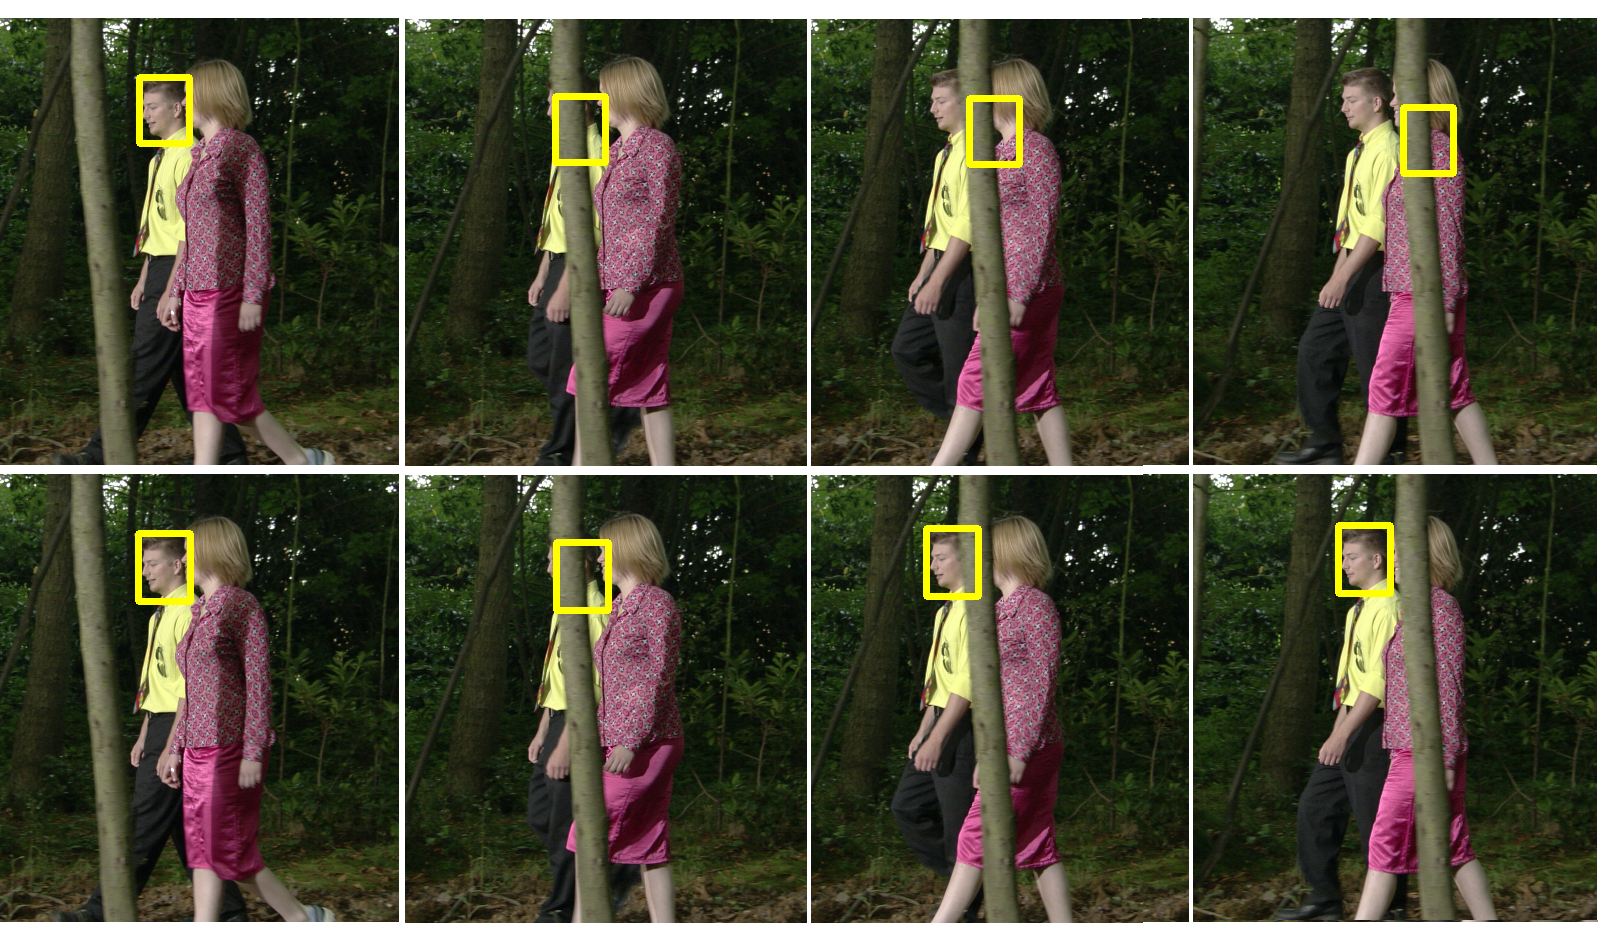
\includegraphics[width=1.0\textwidth]{../images/struckComp.png}
      \caption{Struck tracker in the Walking Couple sequence. Top: Original Implementation. Bottom: Struck tracker with sampling refinement by background regions tracking.}
      \label{tr_strucktest}
   \end{figure}
 
This idea is summarized with the experiment performed with the {\it Struck} tracker. These results can be observed in the Fig. \ref{tr_strucktest}. The sampling process is altered to receive feedback 
from the background segmentation. As it can be seen, for the top row (original implementation using only Haar features) the tracker starts 
learning the tree (oclussion object) since the third shown frame. On the other hand, as the sampling process is modified by rejecting the zones 
labelled as background (including the tree), the tracker quickly recovers after the oclussion in the bottom row. Both experiments were performed 
with a very narrow search window, and by using only Haar features. This is, the tracker did not learn the features extracted 
from the occluding object, and the original object is recaptured when it reappears in the scene. Altough these experimentes are promising, a more deep study is needed, since the {\it Struck} tracker can be more robust if an optimal search window is used, and more features are included in 
the machine learning process.

